
\chapter{Breve introducción al Clustering}\label{ch:Breve introducción al Clustering}

En primer lugar, será necesario realizar una introducción, siquiera sea breve, al clustering y sus aplicaciones, que facilite la comprensión de las siguientes secciones. A tal fin se seguirá el estudio realizado por Brian S. Everitt et al. (2011) \cite{ClusterAnalysis}.

\section{Motivación para la clasificación}

La clasificación puede ser entendida como una forma de simplificar la información contenida en grandes conjuntos de datos, de un modo que sea fácilmente comprensible por las personas. De esta manera, los procesos de extracción de información útil y aplicación de la misma se simplifican. Así, si somos capaces de dividir de forma válida un gran conjunto de datos en subconjuntos o grupos, podremos extraer información común a todos los elementos del subconjunto y proporcionar una descripción precisa de los englobe.

La necesidad de analizar la información de esta manera crece con la aparición y disponibilidad de grandes conjuntos de datos en el ámbito de la ciencia. El análisis de este tipo de información mediante clasificación, o clustering, hoy en día es conocido como \textit{Ciencia de datos}. En el siglo 21 surge un particular interés en la ciencia de datos desde la aparición de la \textit{World Wide Web}, conocida como Internet, donde el objetivo se ha convertido en extraer información relevante de las páginas Web que forma esta basta red.

Es importante destacar que en la mayoría de las ocasiones no hay un sólo criterio de clasificación para un mismo conjunto de datos, de hecho existe una amplia variedad de los mismos. En el caso de las personas, podrían ser clasificadas, por ejemplo, en base a sus ingresos económicos, o según la cantidad de calorías que consumen a lo largo de un periodo de tiempo definido. Así, distintos criterios de clasificación no tiene porque dar como resultado la misma división en grupos del conjunto a clasificar, de esta manera, diferentes criterios servirán a diferentes propósitos.

\section{Métodos numéricos para el Clustering}

Los métodos numéricos para el clustering surgen en ramas de las ciencias naturales, como la biología o la zoología, en un intento de eliminar la subjetividad implícita en el proceso de clasificación que se desencadena al descubrir una nueva especie. El objetivo es proporcionar un método no subjetivo y estable para clasificar y agrupar elementos.

Estos métodos adoptan diversos nombres que varían según el campo en el que se apliquen, taxonomía numérica (\textit{numerical taxonomy}) en biología, $Q$ análisis (\textit{$Q$ analysis}) en psicología, o reconocimiento de patrones no supervisado (\textit{unsupervised pattern recognition}) en el campo de la inteligencia artificial. No obstante, hoy en día, análisis de clusters (\textit{Clusters analysis}) o simplemente clustering son los términos más ampliamente aceptados y extendidos para referirse a tareas que involucran el descubrimiento de subgrupos dentro de un conjunto de elementos.

En la mayoría de las aplicaciones del clustering, el objetivo es obtener una partición de los datos, en la que cada instancia u objeto pertenezca a un único cluster, y la unión de todos ellos contenga a todos los objetos individuales. Dicho esto, debe destacarse que en algunas circunstancias son aceptables soluciones en las que existe solapamiento entre clusters, así como el hecho de que puede no existir una partición aceptable de los datos.

La manera más ampliamente extendida de representar la información sobre la que se debe aplicar clustering es una matriz $X$ de dimensión $n\times p$, en la que cada fila corresponde a una instancia u objeto a procesar, y cada columna corresponde a una de las variables que caracterizan dichas instancias u objetos. El término comúnmente aceptado para referirse a cada fila es el de \textit{vector de características}.


$$ X = \left( \begin{array}{cccc}

x_{1,1} & x_{1,2} & \cdots & x_{1,p} \\

x_{2,1} & \cdots & \cdots & \cdots  \\

\vdots & \vdots & \vdots & \vdots \\

x_{n,1} & \cdots & \cdots & x_{n,p} \\

\end{array} \right) $$

La entrada $x_{i,j}$ en $X$ se corresponde con el valor de la variable $j$-esima en la instancia $i$.

Las variables en $X$ pueden ser una mezcla de atributos en un dominio continuo, discreto o categórico. Además, es posible que, en problemas reales, algunas entradas no estén disponibles. Esta mezcla de tipos de variables y los valores perdidos pueden complicar la tarea del clustering, sin embargo, existen métodos para tratar estos casos, como la inferencia de valores perdidos o las transformaciones de dominio.

En algunas aplicaciones, las filas de la matriz pueden contener medidas repetidas de la misma variable, aunque bajo diferentes condiciones, o en diferentes momentos, incluso en diferentes localizaciones espaciales. Un ejemplo de ello pueden ser las medidas de altura de un grupo de niños en un mismo mes a lo largo de diferentes años. Este tipo de datos poseen una estructura que, de nuevo, puede complicar la tarea del clustering.

Algunos métodos de clustering conllevan realizar transformaciones sobre la matriz $X$ para transformarla en una matriz de $n \times n$ en la que se almacenan medidas extraídas de la matriz $X$ que relacionen una instancia con todas las demás, como pueden ser la similitud, distancia o disimilitud.

El clusterign es, dicho de manera simple, descubrimiento de grupos en datos, y no debe ser en ningún caso confundido con los métodos de discriminación o asignación, conocidos en el ámbito de la inteligencia artificial como aprendizaje supervisado, en los que los grupos son conocidos a priori y el objetivo del análisis es obtener una regla de clasificación o clasificador que permita asignar nuevas instancias o individuos a uno de los grupos ya conocidos.


Una vez definida la estructura general de los métodos de clustering, estaría justificado preguntar, ¿qué es un cluster? La siguiente sección (\ref{QueEsCluster}) intentará dar respuesta a esta pregunta.

\subsection{¿Qué es un cluster?} \label{QueEsCluster}

Hasta este momento, los términos cluster, grupo y clase han sido empleados de una manera completamente intuitiva, sin necesidad alguna de definición formal, una prueba más de lo innato de estos conceptos en el ser humano. De hecho, dar una definición formal de cluster resulta una tarea, no solo complicada, sino en muchas ocasiones poco útil. Bonner, por ejemplo, en 1964 propuso una definición de cluster completamente dependiente de la interpretación del usuario, en lo que a él respecta, un cluster es aquello que el usuario entiende como cluster sin haberle propuesto una definición formal del mismo.

Aunque la definición de Bonner es acertada en una amplio rango de situaciones, autores como Cormack, en 1971, o Gordon en 1999, proponen una definición algo más analítica desde el punto de vista matemático, definiendo un cluster en términos de cohesión interna (homogeneidad), y aislamiento externo (separación). La figura 2.1 muestra, de manera informal, las propiedades descritas anteriormente, de forma que, a cualquier observador, le resultarán aparentes los clusters presentes en ella, sin necesidad de una definición formal de cluster. Este hecho puede explicar porqué alcanzar una definición matemáticamente precisa de homogeneidad y separación puede llegar a ser innecesario.

No queda completamente clara la manera en que las personas reconocen diferentes clusters cuando estos son representados en un plano, pero una de las variables que con certeza influye es la distribución de distancias relativas entre los objetos o puntos.

\clearpage

\begin{figure}[bth]
	\myfloatalign
	{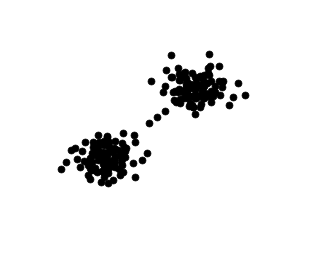
\includegraphics[width=.3\linewidth]{imagenes/c2/TwoBasicsClusters}}
	{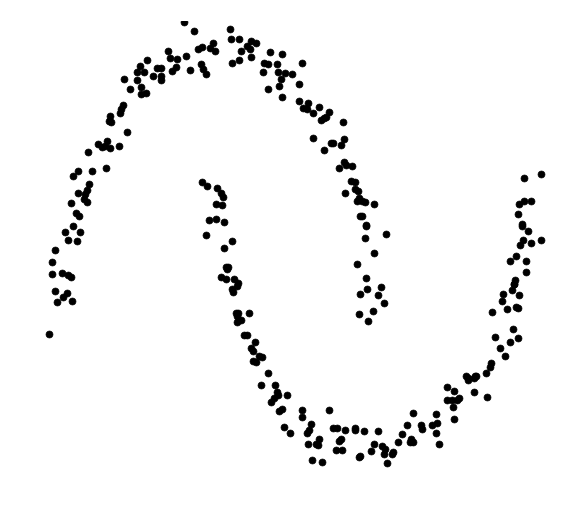
\includegraphics[width=.3\linewidth]{imagenes/c2/MoonsBasics}}
	{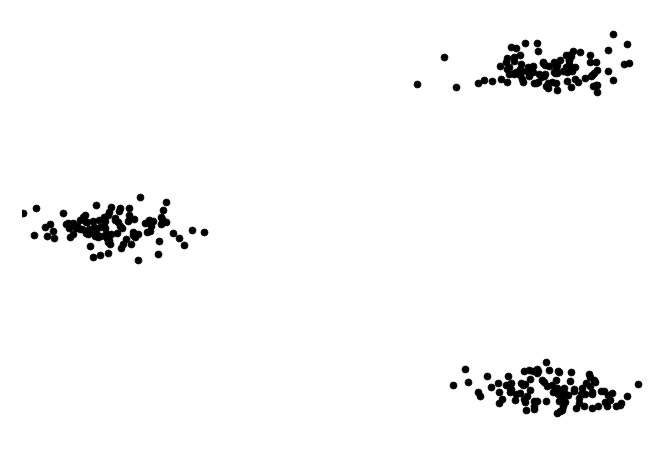
\includegraphics[width=.3\linewidth]{imagenes/c2/ThreeBasicClusters}}
	\caption[Clusters con cohesión interna y/o aislamiento externo]{Clusters con cohesión interna y/o aislamiento externo}\label{fig:figure1}
\end{figure}

Por otra parte, como ya mencionamos anteriormente en esta sección, pueden existir conjuntos de datos en los que no exista una partición justificada. En la figura 2.2 se muestra un conjunto de datos para el que la mayoría de observadores llegaría a la conclusión de que no existen grupos diferenciados, simplemente una nube de puntos uniformemente distribuida. Idealmente, es de esperar que un método de clustering aplicado a este mismo conjunto de datos llegue a la misma conclusión.

\begin{figure}[!h]
	\centering
	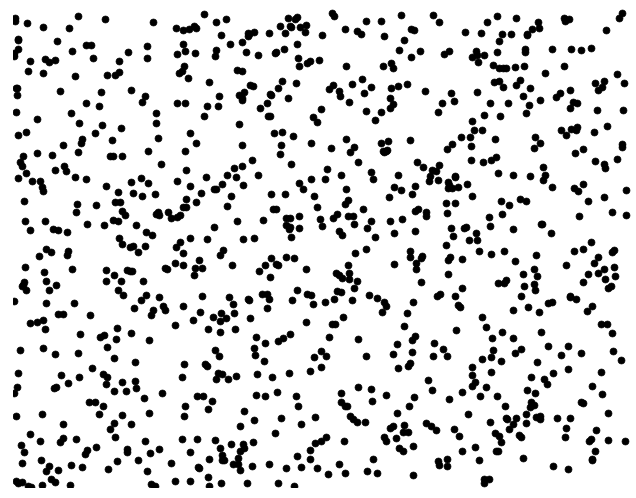
\includegraphics[scale=0.2]{imagenes/c2/rand.png} 
	\caption{Distribución uniforme de puntos}\label{fig:figure2}
\end{figure}

Sin embargo, la mayoría de métodos de aprendizaje no supervisado darán como resultado un particionamiento uniforme como el que se muestra en la figura 2.3. El número de particiones encontrado dependerá del método aplicado, si bien en cualquier caso obtendremos un particionamiento uniforme.

\begin{figure}[!h]
	\centering
	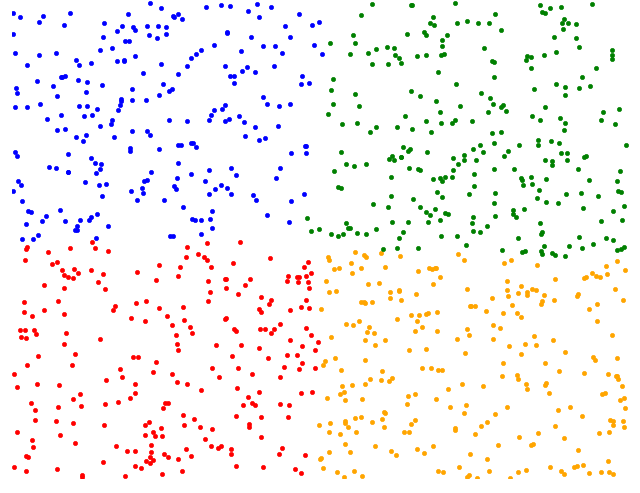
\includegraphics[scale=0.2]{imagenes/c2/randClasif.png} 
	\caption{Distribución uniforme de puntos clasificados}\label{fig:figure3}
\end{figure}

El proceso de dividir una distribución homogénea de datos en diferentes grupos se conoce como disección, y tal proceso puede ser útil en ciertas circunstancias. Sin embargo, dado que en la mayoría de las ocasiones de aplicación real de métodos de clusters no se conoce a priori la estructura de los datos, existe el riesgo de interpretar todas las soluciones en términos de existencia de subgrupos, lo que conllevaría a la imposición de una estructura ficticia en datos en los que no hay estructura presente.

\section{Aplicaciones del clustering}

Como ya se ha indicado, el problema general al que el intenta dar solución el clustering está presente en muchas disciplinas de la ciencia: biología, botánica, medicina, psicología, geografía, marketing, procesamiento de imágenes, psiquiatría, arqueología, etc. En esta sección se presentan algunas de las aplicaciones del clustering relacionadas con las citadas disciplinas.

\subsection{Aplicaciones en marketing}

Dividir los clientes en grupos homogéneos es una de las tareas mas frecuentes en marketing. Un director de marketing podría preguntarse como agrupar los posibles clientes según los beneficios potenciales del producto que intenta introducir en el mercado. Por otra parte, un analista de marketing podría estar interesado en agrupar las empresas según sus características financieras, para poder analizarlas y predecir sus estrategias de mercado.

Un ejemplo de aplicación del clustering en este ámbito fue publicado en Green et al. (1967). Así, con un gran número de ciudades disponibles para el análisis, debieron restringir los lugares en los que llevar a cabo sus estudios, debido a motivos económicos. Para ello hicieron uso del análisis de clusters, clasificando las ciudades en pequeños grupos basándose en 14 características de las mismas, entre ellas se encontraban el tamaño e ingresos medios \textit{per capita}. Dado que se esperaba que las ciudades incluidas en un mismo grupo fueran muy similares, escogieron una ciudad de cada uno de ellos para realizar sus estudios.

Otra aplicación del análisis del clusters en el marketing fue descrita por Chakrapani (2004). En este caso, un fabricante de coches cree que comprar un coche deportivo no es una decisión basada sólo en capacidades económicas o edad, sino que es una decisión relacionada con el estilo de vida que llevan aquellos que deciden comprar un coche de estas características, frente a aquellos que no lo hacen. Consecuentemente, el fabricante decide realizar un estudio, empleando análisis de clusters, que le permita identificar todas las características relacionadas con las personas que comprarían un coche deportivo, para así enfocar sus campañas de marketing a este sector específicamente.

\subsection{Aplicaciones en astronomía}

Dado un conjunto de datos astronómicos, los investigadores quieren saber, por ejemplo, cuantas clases de estrellas hay presentes en ellos, basándose en algun criterio estadístico. Las preguntas más frecuentes dentro de este ámbito son: ¿Cuantos objetos estadísticamente diferentes están presentes en los datos y a que clase debe ser asignado cada objeto? ¿Aparecen clases de objetos previamente desconocidas?. El análisis de clusters puede ser aplicado para dar respuesta a estas cuestiones, ayudando a detectar objetos estadísticamente anómalos, así como a guiar el proceso de clasificación de los mismos. Algunos ejemplos incluyen el descubrimiento de quasars con alto corrimiento al rojo, quasars de tipo 2 (altamente luminosos, núcleos galácticos activos a menudo oscurecidos por polvo y gas), y enanas marrones.

Un ejemplo específivo viene dado por el estudio de Faúndez-Abans et al. (1996), que aplicó técnicas de clustering a datos sobre la composición química de 192 nebulosas planetarias. Se identificaron 6 grupos diferentes que eran similares en muchos aspectos a una clasificación previa de dichos objetos, pero que también mostraban diferencias interesantes que hasta ese momento los investigadores había pasado por alto.

Un segundo ejemplo lo encontramos en el estudio de Celeux y Govaert (1992), quienes aplicaron cluster basado en distribuciones normales a un conjunto de 2370 estrellas, descritas por su velocidad relativa al núcleo galáctico y a la rotación galáctica. Usando un modelo de tres clusters, encontraron un cluster de gran tamaño y pequeño volumen, y dos de pequeño tamaño y gran volumen.

\subsection{Aplicaciones en psiquiatría}

Las enfermedades de la mente son a menudo más difíciles de diagnosticar que las enfermedades del cuerpo, es por ello que en el campo de la psiquiatría ha crecido el interés por las técnicas de análisis de clusters que permitan refinar, o incluso redefinir, las técnicas de diagnosis para este tipo de enfermedades. Gran parte de este trabajo involucra pacientes deprimidos, en los que el interés reside en distinguir entre dos tipos de depresión, la endógena (congénita), y la neurótica.

Pilowsky et al. (1968), por ejemplo, usando métodos desarrollados por otros autores, aplicó técnicas de clustering a 200 pacientes en base a sus respuestas a un cuestionario sobre la depresión, junto a información sobre su sexo, edad, estado mental y enfermedad padecida. Este es un claro ejemplo de variables de diferentes tipos incluidas en el mismo conjunto de datos. Uno de los grupos obtenidos como resultado de este estudio fue identificado como marcador de la depresión endógena.

El análisis de clusters también ha sido empleado para encontrar una clasificación de individuos que intentaron cometer suicidio, que podría sentar las bases para estudios posteriores sobre las causas y tratamientos del problema. Paykey y Rassaby (1978), por ejemplo, estudiaron 236 casos de suicidas fallidos registrados por el servicio de emergencias de una ciudad de los Estados Unidos de América. Del conjunto de las variables posibles, 14 fueron seleccionadas como particularmente relevantes para la clasificación, y por tanto fueron usadas en el análisis. Entre ellas se encontraban la edad, numero de intentos de suicidio, gravedad de la depresión, grado de hostilidad, además de na serie de características demográficas. Al conjunto de datos resultante se le aplicaron métodos de clustering, el resultado mas significativo obtenido corresponde a una división en tres clusters bien definidos.

\subsection{Aplicaciones en meteorología y climatología}

Diariamente se recogen enormes cantidades de datos sobre la meteorología mundial, explorar estos datos mediante técnicas de clustering puede aportar nuevos enfoques para la climatología y el medio ambiente.

Littmann (2000), por ejemplo, aplicó clustering a los datos recogidos sobre los cambios diarios en la presión superficial en la cuenca Mediterránea, y encontró 20 grupos que explicaban la varianza de las lluvias en las regiones centrales del Mediterráneo. Otro ejemplo viene de la mano de Liu y George (2005), quienes usaron el algoritmo \textit{fuzzy k-means} a datos espaciotemporales de la climatología de las regiones del sur central de EEUU. 

\subsection{Aplicaciones en arqueología}

La arqueología es otra de las disciplinas en la que resulta útil la aplicación del clustering. La clasificación de los diferentes objetos encontrados en los yacimientos puede ayudar a descubrir su uso, los periodos a los que pertenecen, así como la población que los utilizó. De forma similar, el estudio de materiales fosilizados puede ayudar a revelar como vivieron las sociedades prehistóricas. 

Un ejemplo temprano de la aplicación de clustering a objetos arqueológicos viene dado por Hodson et al. (1966), que aplicó técnicas de clustering a un grupo de broches que datan de la Edad de Hierro, encontrando una clasificación para los mismos de demostrada relevancia arqueológica. Otro ejemplo de la mano de Hodson (1971) es la aplicación del algoritmo \textit{k-means} para construir una taxonomía de hachas de mano encontradas en las Islas Británicas. Las variables tenidas en cuenta para describir cada hacha incluyen longitud, anchura y valores en una escala que describen cómo de puntiaguda era la herramienta. El clustering dio como resultado dos grupos de hachas, uno formado por las pequeñas y delgadas, y otro formado por las grandes y gruesas.

Respecto a materiales fosilizados, Sutton y Reinhard (1995) realizaron un estudio sobre 155 coprolitos encontrados en \textit{Antelope House}, un yacimiento prehistórico en el Cañón de Chelly en Arizona. El estudio arrojó como resultado en una interpretación de las diferencias entre coprolitos basada en la alimentación.

\subsection{Aplicaciones en bioinformática y genética}

Tiempos recientes están siendo testigo de un tremendo crecimiento en el interés por la Bioinformática, acompañada por la biología molecular, ciencias de la computación, matemáticas y estadística. Tal crecimiento ha sido acelerado por la siempre creciente base de datos genómica y proteica, que son por sí mismas resultado de un grandísimo avance en las técnicas de secuenciación del ADN, medidas de expresión de los genes y compresión de las estructuras macromoleculares. La estadística ha jugado un papel relevante en el estudio de la expresión de los genes. Los genes contenidos en el ADN de cada célula proporcionan las plantillas necesarias para la generación de las proteínas implicadas en la mayoría de los procesos estructurales y biomecánicos que tienen lugar en cada uno de nosotros. Sin embargo, aunque la mayoría de las células en los seres humanos contiene todos los complementos genéticos que componen el genoma humano, los genes se expresan de manera selectiva en cada célulan dependiendo del tipo de la misma, del tejido y de las condiciones generales tanto dentro como fuera de la célula. La biología molecular ha puesto de manifiesto que la mayoría de los procesos en la vida de una célula están regulados por factores que afectan a la expresión de sus genes.

Como hemos visto, uno de los campos de investigación mas activos hoy en día es el que estudia los procesos que regulan la expresión de los genes. Con el fin de almacenar la información relativa a esta área de estudio surgen los microarrays, (Cortesse, 2000). Desde el punto de vista del análisis de datos, una de las características relevantes en este tipo de información es que el número de características de cada instancia ($p$), supera con creces al número de instancias disponibles ($n$); cojuntos de datos como este son calificados como \textit{datos de alta dimensionalidad}.

La mayoría de métodos estadísticos clásicos no pueden ser aplicados a este tipo de conjuntos de datos sin ser modificados de forma sustancia. Sin embargo, el análisis de clusters acepta bien tales conjuntos de datos y puede ser empleado para identificar grupos de genes con patrones de expresión similares, y dar respuesta a preguntas como porqué un gen se ve afectado por cierta enfermedad, o qué genes son responsable de enfermedades genéticas hereditarias.

Un ejemplo de aplicación lo encontramos en el trabajo de Selinski e Ickstadt (2008), quienes usaron clustering sobre polimorfismos de nucleótidos simples para detectar diferencias entre enfermedades a nivel genético.

\section{Resumen}

Las técnicas de clustering consisten en la exploración de conjuntos de datos sobre los que se debe discernir si pueden o nor ser resumidos de manera significativa en términos de un número relativamente pequeño de grupos o clusters de objetos o individuos que se parecen unos a otros y que se diferencian de los que se encuentran en otros clusters.

Muchas ramas de la ciencia han hecho uso de las técnicas de clustering, de manera exitosa, para avanzar en sus respectivos campos y procesar grandes cantidades de datos, cuyo análisis sería impensable afrontar con otras técnicas.

%\let\cleardoublepage\relax

%Para referir un acronimo completo \acf
%Para referir un acronimo solo con las siglas \acs




















